%Matteo Kumar - Leonhard Schatt
% Fortgeschrittenes Physikalisches Praktikum

% Teilauswertung Oberflächengitter
\clearpage
\section{Gitterkonstante eines Oberflächengitters}

Als letzes wird noch ein Oberflächengitter vermessen, um dessen Gitterkonstante zu bestimmen. Dazu wird wieder ein Profil entlang der in 
Abb. \ref{bild:OFGitter} eingezeichneten Linie erstellt.

\begin{figure}[h]
    \centering
    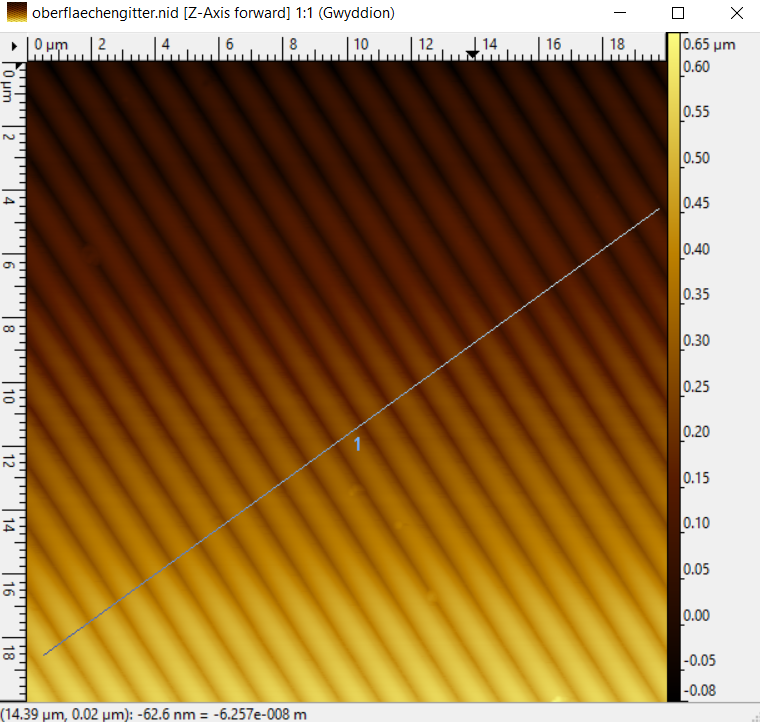
\includegraphics[scale = 0.45]{Bilder/OFGitter.png}
    \caption{Höhenprofil der ersten Geraden}
    \label{bild:OFGitter}
\end{figure}

\begin{figure}[ht]
    \centering
    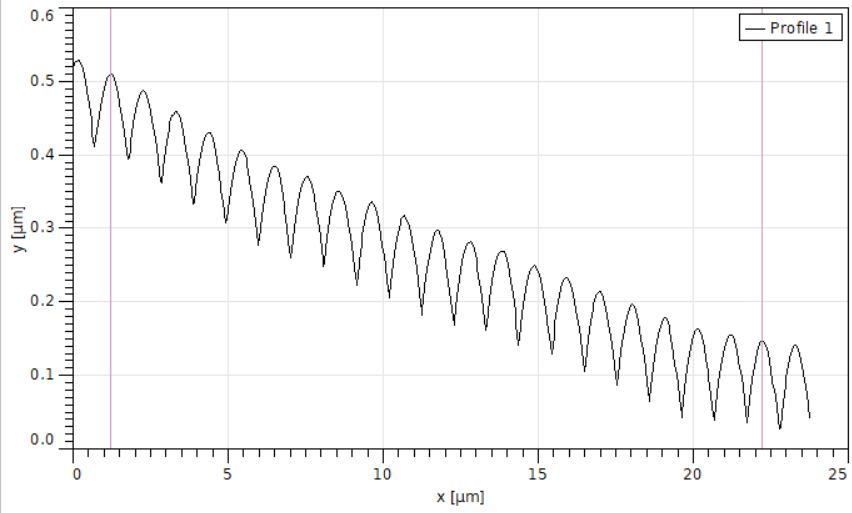
\includegraphics[scale = 0.55]{Bilder/OFGitterProfil.png}
    \caption{Höhenprofil der ersten Geraden}
    \label{bild:OFGitterProfil}
\end{figure}


Anschließend wird das Profil über 20 Kanten hinweg vermessen, wie in Abb. \ref{bild:OFGitterProfil} gezeigt. Die Gesamtlänge beträgt 
21.016 $\mu$m; der Mittelwert beträgt also 1.0508$\mu$m. 
Der Fehler liegt wieder in dem Setzen der Linien, zwischen denen gemessen wurde. Anhand des Abmess-Tools wird dieser auf 0.1$\mu$m pro 
Linie geschätzt. Für den Mittelwert ergibt sich demnach ein Fehler von 0.01$\mu$m. Die Gitterkonstante des Oberflächengitters beträgt also:
\begin{equation*}
    \textcolor{red}{g = (1.05 \pm 0.01) \mu m}
\end{equation*}